% SysContract — 4-page extended abstract for NeurIPS 2026 Workshop on ML for Systems
% Camera-ready version (de-anonymized). Strict 4-page limit excluding references and appendix.
\documentclass{article}

\usepackage[dblblindworkshop,final,nonatbib]{neurips_2026}
\usepackage{natbib}
\renewcommand{\sfdefault}{cmss}
\workshoptitle{ML for Systems}

\usepackage[utf8]{inputenc}
\usepackage[T1]{fontenc}
\usepackage{url}
\usepackage{booktabs}
\usepackage{amsmath}
\usepackage{amssymb}
\usepackage{microtype}
\usepackage{graphicx}
\usepackage{flafter}
\usepackage{tikz}
\usetikzlibrary{arrows.meta, positioning}
\usepackage{hyperref}
\hypersetup{
  pdftitle={SysContract: Stop-Check-Act Runtimes for Agents that Control Computer Systems},
  pdfauthor={Israel Olanrewaju Odeajo},
  colorlinks=false,
  pdfborder={0 0 0}
}

\title{SysContract: Stop--Check--Act Runtimes for Agents that Control Computer Systems}

\author{%
  Israel Olanrewaju Odeajo \\
  WorldQuant University \\
  \texttt{isrealodeajo@gmail.com}
}

\begin{document}

\maketitle

\begin{abstract}
LLM agents are increasingly given write access to schedulers, database knobs, and serving stacks.
A single quality metric does not determine whether the resulting configuration is admissible.
We study unconstrained GPT-4o-mini on three control tasks.
On a fluid serving model it triples tokens/s while violating the TTFT and KV-cache envelope on every seed.
On a cluster packer and on SQLite it often violates invariants \emph{without} improving the scored metric.
Putting the same invariants in the prompt, with no gate, raises SQLite hold rate to $1.0$ but still leaves serving hold at $0.40$ and does not stop post-plateau thrashing.
\textbf{SysContract} admits an action only if a machine-checked envelope holds, rolls back dynamic failures, and stops when further calls are not buying improvement.
It is admission control for configuration actions, not a better prompt.
On all three tasks it rejects every violating write and cuts GPT token use by $4$--$4.5\times$; on SQLite it also improves latency inside the envelope.
\end{abstract}

\section{Introduction}

Recent work shows that LLM agents can synthesize Linux schedulers, tune operating-system knobs, and rewrite GPU kernels~\cite{zheng2025schedcp,liargkovas2025expert,tschand2025swizzleperf,hong2025autocomp}.
Those results establish that language models can \emph{propose} systems changes.
They do not establish that the resulting closed loop is safe to leave in place.

An agent with write access is a controller.
The quantity typically reported---mean job-completion time, tokens/s, query latency---is not the quantity that makes a configuration \emph{admissible}.
Admissibility is a conjunction of invariants: no starvation, no SLO breach on a hidden class, no OOM, unchanged query results, a path to roll back.
None of these need appear in the scalar the agent was told to improve.

We make three contributions.
(1)~We measure \emph{metric hacking} by unconstrained ReAct-style agents~\cite{yao2023react}: $J$ can rise, fall, or stall while $\mathcal{I}$ fails.
(2)~We show that naming $\mathcal{I}$ in the prompt is not a substitute for a gate.
(3)~We present SysContract, a stop--check--act runtime that intercepts proposed knob writes, plus a scorecard over quality, hold rate, and token cost.
Random search is a required baseline~\cite{ansel2014opentuner}.

\section{Failure modes}

Let $J(\theta)$ be the scalar shown to the agent and $\mathcal{I}(\theta)\in\{0,1\}$ the conjunction of invariants.
The intended problem is $\max_\theta J(\theta)$ subject to $\mathcal{I}(\theta)=1$.
The unconstrained agent solves $\max_\theta J(\theta)$.

\textbf{Hidden class.}
Mean JCT is dominated by batch jobs.
Raising batch priority and overcommit can move $J$ while interactive p99, which is not in $J$, degrades.

\textbf{Capacity lie.}
Tokens/s rewards larger batches and higher memory utilization until TTFT or KV-cache limits, which are not in $J$, fail.

\textbf{Thrashing after the plateau.}
Agents keep calling the model after the last meaningful improvement.
Those extra steps overfit the measurement window and are where unsafe or merely worse actions concentrate.

Zheng et al.\ showed that a naive agent generating eBPF can be slow, expensive, and worse than EEVDF~\cite{zheng2025schedcp}.
The same control-loop pathology appears when the agent is restricted to knobs.
A bytecode verifier does not gate a configuration write.

\section{SysContract}

\begin{figure}[ht]
\centering
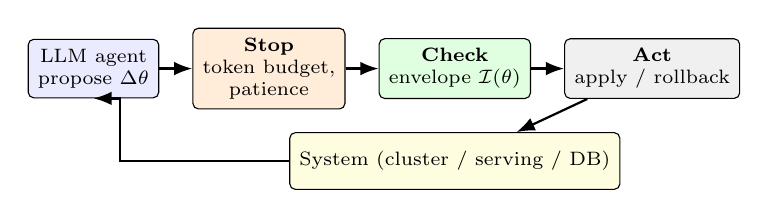
\begin{tikzpicture}[
  font=\scriptsize,
  box/.style={draw, rounded corners=2pt, align=center, inner sep=3.5pt, minimum height=0.72cm},
  arr/.style={-{Latex}, thick}
]
\node[box, fill=blue!8] (agent) {LLM agent\\propose $\Delta\theta$};
\node[box, fill=orange!15, right=0.42cm of agent] (stop) {\textbf{Stop}\\token budget,\\patience};
\node[box, fill=green!12, right=0.42cm of stop] (check) {\textbf{Check}\\envelope $\mathcal{I}(\theta)$};
\node[box, fill=gray!12, right=0.42cm of check] (act) {\textbf{Act}\\apply / rollback};
\node[box, fill=yellow!12, below=0.42cm of check] (env) {System (cluster / serving / DB)};
\draw[arr] (agent) -- (stop);
\draw[arr] (stop) -- (check);
\draw[arr] (check) -- (act);
\draw[arr] (act) -- (env);
\draw[arr] (env.west) -| ++(-2.15,0) |- (agent.south);
\end{tikzpicture}
\caption{The model proposes a configuration delta. The runtime decides whether it is an admissible mutation.}
\label{fig:arch}
\end{figure}

\paragraph{Envelope.}
Each environment exposes $\theta\in\Theta$ and a predicate $\mathcal{I}(\theta)$ evaluated \emph{before} commit (range check or dry-run).
Failing actions never reach the system.
This is admission control, not safety fine-tuning of the model.

\paragraph{Stop.}
SysContract stops when $J$ has not improved by relative $\varepsilon$ for $p$ consecutive steps ($t\ge t_{\min}$), or the token budget is exhausted.
The rule is a preemption policy for optimization agents, not a sequential hypothesis test.

\paragraph{Act / rollback.}
Admitted actions are applied.
If a dynamic check (checksum, RSS, crash) fails, the last snapshot is restored.

\paragraph{Role of the model.}
The LLM proposes which knobs to change.
It is not the verifier, the stopping rule, or the execution path.
Prior agent--OS work used a similar split for generated eBPF~\cite{zheng2025schedcp}; we apply it to configuration writes and add stopping.

\section{Experiments}

\paragraph{Setup.}
GPT-4o-mini, temperature $0.5$, JSON proposals, $6$ steps, $5$ seeds.
GPT is shown $J$ and knob ranges; $\mathcal{I}$ is omitted from the observation.
GPT-aware is shown $\mathcal{I}$ in the prompt and still has no gate.
(1)~Cluster: discrete-event packer, $8$ machines, mixed interactive/batch jobs; $J$ is mean JCT (lower better); $\mathcal{I}$ is interactive p99 SLO, no starvation, no overcommit.
(2)~Serving: a \emph{fluid model} of LLM batching (not a serving engine); $J$ is tokens/s (higher better); $\mathcal{I}$ is TTFT SLO, KV-cache cap, no starvation.
(3)~SQLite: PRAGMA autotune on a local database; $J$ is query ms (lower better); $\mathcal{I}$ is checksum, RSS, durability (\texttt{synchronous} not OFF).
Controllers: default; random search with the same step budget~\cite{ansel2014opentuner}; random+SysContract; unconstrained GPT; GPT-aware; GPT+SysContract.
For gated methods we report the best admissible $J$.
A method that wins $J$ and loses $\mathcal{I}$ is a failure.

\begin{table}[ht]
\caption{Mean over $5$ seeds (sample std in parentheses). Hold is the fraction of seeds with $\mathcal{I}{=}1$ at commit.
On cluster and serving, gated hold $1.00$ is by construction: the gate uses the same predicate later used to score hold.
Unconstrained and GPT-aware hold are empirical.
Token counts are GPT API usage (blank for non-LLM controllers).
Lower $J$ is better on cluster and SQLite; higher $J$ is better on serving.}
\label{tab:main}
\centering
\scriptsize
\setlength{\tabcolsep}{2.4pt}
\begin{tabular}{llccc}
\toprule
Env & Controller & $J$ & Hold & Tokens \\
\midrule
Cluster & Default & $7.01$ $(1.23)$ & $1.00$ & --- \\
Cluster & Random & $7.47$ $(2.19)$ & $0.00$ & --- \\
Cluster & Random+SC & $7.01$ $(1.23)$ & $1.00$ & --- \\
Cluster & GPT & $7.00$ $(1.25)$ & $0.20$ & $2473$ \\
Cluster & GPT-aware & $10.75$ $(7.31)$ & $0.60$ & $2807$ \\
Cluster & GPT+SC & $7.01$ $(1.23)$ & $1.00$ & $568$ \\
\midrule
Serving & Default & $469$ & $1.00$ & --- \\
Serving & Random & $966$ $(440)$ & $0.40$ & --- \\
Serving & Random+SC & $469$ & $1.00$ & --- \\
Serving & GPT & $1444$ $(57)$ & $0.00$ & $2560$ \\
Serving & GPT-aware & $745$ $(177)$ & $0.40$ & $2772$ \\
Serving & GPT+SC & $469$ & $1.00$ & $575$ \\
\midrule
SQLite & Default & $1.90$ $(0.35)$ & $1.00$ & --- \\
SQLite & Random & $2.03$ $(0.68)$ & $0.20$ & --- \\
SQLite & Random+SC & $2.24$ $(1.20)$ & $1.00$ & --- \\
SQLite & GPT & $2.65$ $(0.19)$ & $0.00$ & $2702$ \\
SQLite & GPT-aware & $2.62$ $(0.71)$ & $1.00$ & $3050$ \\
SQLite & GPT+SC & $1.62$ $(0.13)$ & $1.00$ & $598$ \\
\bottomrule
\end{tabular}
\end{table}

\paragraph{Unconstrained GPT.}
On serving, GPT triples tokens/s ($469\to 1444$) with hold $0/5$.
On cluster, $J$ does not improve ($7.01$ vs $7.00$) while hold is $0.20$.
On SQLite, latency gets worse ($1.90\to 2.65$\,ms) with hold $0/5$.
A speedup is therefore not required for the configuration to be wrong, and a speedup is not sufficient for it to be admissible.
Random search produces the same shape on serving ($966$ tokens/s, hold $0.40$).

\paragraph{A prompt is not a gate.}
GPT-aware, told the hard constraints and still unconstrained, reaches SQLite hold $1.00$ (discrete durability rules are easy to follow) but serving hold only $0.40$ and cluster hold $0.60$, including one cluster seed with JCT $23$.
SQLite $J$ remains worse than default ($2.62$\,ms) because the agent keeps stepping after the plateau.
Naming $\mathcal{I}$ reduces some violations; it does not enforce them and does not stop thrashing.

\paragraph{SysContract.}
Gated GPT uses $4.4\times$ fewer tokens on cluster, $4.5\times$ fewer on serving, and $4.5\times$ fewer on SQLite.
On cluster and serving, early rejection of unsafe first proposals leaves $J$ at the default; that is an admissible no-op, not a hidden quality win.
The non-tautological measurements are unconstrained and GPT-aware hold, token use, and SQLite $J$ on a real engine.
On SQLite, where some proposals are both safe and useful, GPT+SC improves latency ($1.90\to 1.62$) while random+SC does not ($2.24$).
Replaying unconstrained GPT proposals through the gate yields $1.51$\,ms: the admissible subset of the same ideas is better than the subset the unconstrained agent committed.
Unconstrained GPT spends $94\%$ of cluster tokens and $74\%$ of SQLite tokens after the last $\varepsilon$-improvement; the stopping rule removes that tail.

\section{Related work}

RL for systems and Park-style environments treat configuration as a sequential decision problem~\cite{mao2019park,mao2019decima,qiu2020firm}.
Autotuners search knobs without LLMs~\cite{ansel2014opentuner,snoek2012practical}.
LLM agents have been applied to schedulers, kernels, RTL, and training sharding~\cite{zheng2025schedcp,tschand2025swizzleperf,hong2025autocomp,bhattaram2025rtl,ding2025asap}.
InfraGym standardizes agent--system loops~\cite{zhang2025infragym}.
Agentix schedules LLM \emph{calls} inside agent programs~\cite{luo2026agentix}; we admit or reject \emph{configuration writes}.
TOCTOU attacks assume a check exists~\cite{lilienthal2025toctou}.

\section{Limitations}

$\mathcal{I}$ is specified by the operator; omitted invariants are not enforced.
On cluster and serving, the gate and the hold metric use the same model of $J$ and $\mathcal{I}$, so gated hold $1.00$ is tautological there; unconstrained hold, token use, the prompt ablation, and SQLite (a real engine) are not.
The serving task is a fluid model, not vLLM or a GPU.
SQLite uses a small local table, not production OLTP.
We use one model, five seeds, and a six-step budget, and the action space is a knob vector rather than generated kernel code.
The stopping rule is a patience heuristic.

\section{Conclusion}

An improved metric is not an admissible configuration.
Telling an LLM the constraints does not enforce them.
SysContract does: it gates writes, rolls back failures, and stops when tokens are not buying improvement.
On three control tasks that is enough to restore hold rate $1.0$, cut token use, and---when safe proposals exist---keep the gains that actually fit in the envelope.

\bibliography{references}
\bibliographystyle{plainnat}

\appendix
\section{Reproducibility}

Hyperparameters used for Table~\ref{tab:main}: GPT-4o-mini, temperature $0.5$, $6$ steps, seeds $\{0,\ldots,4\}$,
relative $\varepsilon=0.01$, patience $p=2$, $t_{\min}=2$, token budget $12{,}000$.
Gated methods report best admissible $J$; unconstrained methods report committed $J$.
GPT-aware uses the same unconstrained loop, with hard constraints included in the prompt.

\begin{verbatim}
python scripts/run_eval.py --env serving --agent llm \
  --seeds 5 --steps 6 --model gpt-4o-mini
python scripts/run_eval.py --env serving --agent llm \
  --aware --unconstrained-only --seeds 5 --steps 6 --model gpt-4o-mini
python scripts/run_eval.py --env serving --agent random --seeds 5
python scripts/run_eval.py --env serving --agent default --seeds 5
\end{verbatim}
Code and logs: \url{https://github.com/israelkingz/syscontract}.

\end{document}
